


\begin{table*}
\caption{Performance (\emph{LFW} Restricted View 2) of the family of biologically-inspired models and blends thereof.} 

\centering
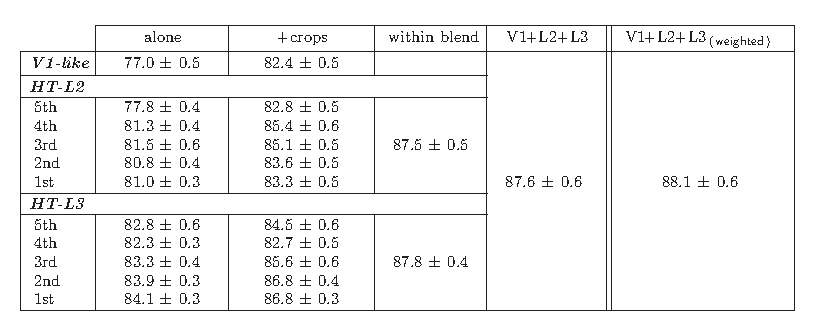
\includegraphics{tables/grand_performance_table_baked.pdf}

\label{tab:grand_performance_table}
\end{table*}





\subsection{High-throughput screening with \emph{LFW} View 1}

Fig. \ref{fig:ht_process} shows the results of high-throughput screening to select
model instantiations that are well-suited to the \emph{LFW} verification task.
For each model class, a multitude of models were randomly generated and
evaluated on the \emph{LFW} view 1 set, and the best five were selected for
further analysis.


\subsection{Performance on \emph{LFW} Restricted View 2}

Performance of individual models and model blends are shown in Table
\ref{tab:grand_performance_table}.  Performance ranging from 77.1 \% for the
simplest \emph{V1-like} model to 88.1\% for the largest blend were observed.  Taken
together, these results show that state-of-the-art level performance is possible
within the model family, and there exist multiple paths (e.g. based purely
on \emph{V1-like} models, and based on high-throughput, multi-layer models) to
achieving high levels of performance.  Fig. \ref{fig:roc_curves} shows
receiver-operator characteristic (ROC) curves for each of these models.

Interestingly, the inclusion of a single additional comparison function to the
\emph{V1-like} model blend described in \cite{pinto:cvpr09} brings an additional
3\% performance, placing it close to the last reported best performance on this
set, even without extensive blending.  Furthermore, we see that individual
\emph{HT-L3} models also perform surprisingly well --- coming to within a few percent correct of
the previous state-of-the-art.

A major advantage of our high-throughput approach is that it produces not one,
but a diversity of models, and this situation is ideally suited to kernel
blending approaches.  Once blending is added, especially when coupled with an
intelligent algorithm for weighting blended kernels, several different blends
achieved performance exceeding previously reported state-of-the-art values (see Figure \ref{fig:table_soa}).  ROC 
curves for various blend groupings are shown in Fig. \ref{fig:roc_curves}.

\begin{figure*}[ht]
\centering 
\subfigure[\small{within-model-class blends}]{
  \includegraphics[scale=0.9]{figures/within_roc.pdf}
  \label{fig:within_rocs}
} 
\subfigure[\small{across-model-class blends}]{
  \includegraphics[scale=0.9]{figures/mega_blend_roc.pdf}
  \label{fig:megablend_rocs}
}
\subfigure[\small{comparison with literature}]{
    \begin{tabular}{|c||c|c|c|c|}
\hline
%Reference & Kumar et al. ICCV09 \cite{kumar:iccv09} & Wolf et al. ACCV09 \cite{wolf:accv09} & Cao et al. CVPR10 \cite{cao2010face} & This paper \\
 & Kumar et al. & Wolf et al. & Cao et al. & \\
Reference & ICCV09 \cite{kumar:iccv09} & ACCV09 \cite{wolf:accv09} & CVPR10 \cite{cao2010face} & This paper\\
\hline\hline 
Mean classification error & 14.7\%$\pm$1.2 & 13.2\%$\pm$0.3 & 15.5\%$\pm$0.5 & \bf{11.9\%$\pm$0.6} \\
\hline 
%\rule{0pt}{2ex}
\end{tabular}
\label{fig:table_soa}
}

\caption[]{{\bf ROC curves for various model sub-families on \emph{LFW}
    Restricted View 2.} Curves for \cite{wolf:accv09}, \cite{kumar:iccv09} and \cite{cao2010face} 
  are plotted in \ref{fig:megablend_rocs} for reference.  Plots are zoomed-in to
  facilitate comparison.}
\label{fig:roc_curves}
\end{figure*}


\subsection{Analysis of Errors}

To understand better where room for improvement lies, we examined the error
trials (misses and false alarms) produced by each model for quantitative and
qualitative trends.  To determine whether different models were primarily making
the same or different errors, we segregated the responses of the \emph{V1-like}
and \emph{HT-L3} models (rescaled-crop augmented variants, see Methods) into
four categories: hits, misses, false positives, and correct rejections.  We then
computed the fraction of errors that these two models held in common and found
84.3\% of false positives were the same across the two models, and that
87.3\% of misses were missed by both models.  This high level of consistency
between error cases across the two models led us to ask whether a subset of
``hard'' images within the larger \emph{LFW} set could be driving errors and
capping performance.

Fig. \ref{fig:error_examples} shows examples of misses and false positives
held in common for both models.  While developing a quantitative framework
within which to analyze these errors is beyond the scope of this paper, several
patterns are evident, even upon casual inspection.  First, misses are dominated
by situations where the individual-to-be-matched is seen in non-frontal view in
at least one of the images.  Second, false positives appear to occur more often
in cases where different individuals appear in a very similar view, or with a
similar expression.


\begin{figure*}[ht]
  \centering \subfigure[Misses]{ 
    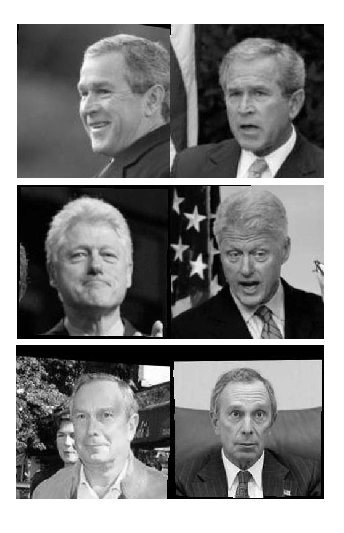
\includegraphics[scale=0.8]{figures/misses.pdf}
    \label{fig:misses}
  } \subfigure[False Positives]{
    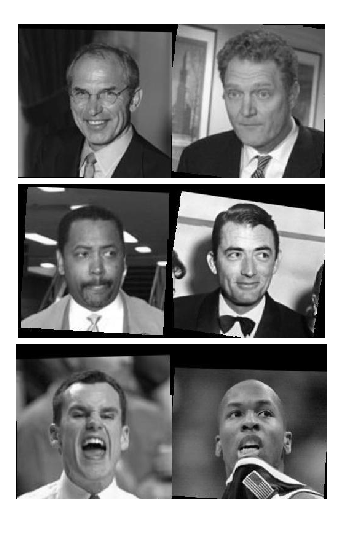
\includegraphics[scale=0.8]{figures/false_positives.pdf}
    \label{fig:false_positives}
  }
  \caption[]{{\bf Examples of common errors across models.} Misses tend to be
    dominated by differences in view, while false positives frequently occur when
    different individuals share a common view or expression. }
  \label{fig:error_examples}
\end{figure*}


 
% \subsection{Performance of models on a synthetic variation ``litmus test'' set}
